
%(BEGIN_QUESTION)
% Copyright 2009, Tony R. Kuphaldt, released under the Creative Commons Attribution License (v 1.0)
% This means you may do almost anything with this work of mine, so long as you give me proper credit

Determine whether moving the potentiometer knob {\it clockwise} will increase or decrease the sensitivity of this analog voltmeter:

$$\includegraphics[width=15.5cm]{i03810x01.eps}$$

\vskip 20pt \vbox{\hrule \hbox{\strut \vrule{} {\bf Suggestions for Socratic discussion} \vrule} \hrule}

\begin{itemize}
\item{} Which way would we need to turn the potentiometer in order to make the voltmeter have a higher range (i.e. full-scale deflection represents a greater measured voltage value than before)
\end{itemize}

\underbar{file i03810}
%(END_QUESTION)





%(BEGIN_ANSWER)

Turning the knob clockwise will {\it decrease} the meter's sensitivity (i.e. make the needle move {\it less} with the same amount of applied voltage at the test lead tips).  This is due to the potentiometer's resistance increasing between the left and center terminals as the wiper sweeps clockwise on the resistive strip.

%(END_ANSWER)





%(BEGIN_NOTES)

%INDEX% Pictorial circuit review (analog voltmeter circuit)

%(END_NOTES)


